\section{Рабочий проект}

В третьей главе были спроектированы архитектура, структура данных и пользовательский интерфейс системы. В данной главе приводится описание реализации разработанной конфигурации: описание процедур и функций, реализация ключевых алгоритмов, результаты функционального тестирования и инструкция по развертыванию.

\subsection{Спецификация программной реализации}

Программная часть системы включает процедуры и функции справочников, документов, форм, общие процедуры и отчеты.

\subsubsection{Процедуры справочников}

Для работы со справочниками системы реализованы процедуры обработки событий записи и проведения. Описание ключевых процедур приведено в таблице 4.1.

\vspace{0.5cm}

\newpage
\noindent
Таблица 4.1 - Процедуры проведения справочников

\vspace{0.2cm}
\noindent
\begin{tabular}{|p{5.75cm}|p{4.5cm}|p{5cm}|}
	\hline
	Процедура & Входные данные & Описание \\
	\hline
	ПередЗаписью (Спортсмены) & Объект справочника & Проверка заполнения обязательных полей (ФИО, дата рождения) \\
	\hline
	ПриЗаписи (Спортсмены) & Объект справочника & Автоматическое формирование наименования по ФИО \\
	\hline
	ПередЗаписью (Тренеры) & Объект справочника & Проверка заполнения специализации (Вид спорта) \\
	\hline
	ПриЗаписи (Тренеры) & Объект справочника & Автоматическое формирование наименования по ФИО \\
	\hline
	ПередЗаписью (Группы) & Объект справочника & Проверка заполнения вида спорта \\
	\hline
	ПриЗаписи (ПериодыВремени) & Объект справочника & Автоматическое формирование наименования по времени начала и окончания \\
	\hline
\end{tabular}

\vspace{0.4cm}

\subsubsection{Процедуры документов}

Для каждого документа реализована процедура обработки проведения, формирующая движения по регистрам. Описание ключевых процедур приведено в таблице 4.2.


\vspace{0.2cm}

\newpage
\noindent
Таблица 4.2 - Процедуры проведения документов

\vspace{0.2cm}
\noindent
\begin{tabular}{|p{5.7cm}|p{5.25cm}|p{4.3cm}|}
	\hline
	Процедура & Формируемые движения & Описание \\
	\hline
	ОбработкаПроведения (РасписаниеЗанятий) & Регистры сведений «Расписание занятий», «Расписание занятий группы» & Обход строк ТЧ, формирование записей для каждого дня недели \\
	\hline
	ОбработкаПроведения (ПриказОНазначении Тренера) & Регистр сведений «Тренер спортсмена» & Запись связки «тренер - спортсмен - вид спорта - дата» \\
	\hline
	ОбработкаПроведения (РезультатыСоревнований) & Регистр сведений «Результаты соревнований» & Обход строк ТЧ, запись результатов \\
	\hline
	ОбработкаПроведения (ПоступлениеИнвентаря) & Регистр накопления «Спортивный инвентарь организации» (приход) & Формирование приходных движений по каждой строке \\
	\hline
	ОбработкаПроведения (ВыдачаИнвентаря) & Регистр накопления «Спортивный инвентарь организации» (расход, приход на МОЛ) & Формирование расходных движений со склада и приходных - на МОЛ \\
	\hline
\end{tabular}
\vspace{0.4cm}

\subsubsection{Процедуры форм}

Формы системы содержат процедуры обработки событий элементов управления. Описание ключевых процедур приведено в таблице 4.3.

\newpage
\noindent
Таблица 4.3 - Процедуры форм

\vspace{0.2cm}
\noindent
\begin{tabular}{|p{5.25cm}|p{3.5cm}|p{6.5cm}|}
	\hline
	Процедура & Форма & Описание \\
	\hline
	ПриСозданииНаСервере & Расписание занятий & Установка текущей даты, инициализация реквизита «Месяц» \\
	\hline
	ПериодПриИзменении & Расписание занятий (общее) & Обновление планировщика при смене периода \\
	\hline
	ТренерПриИзменении & Расписание занятий (общее) & Фильтрация отображения по выбранному тренеру \\
	\hline
	ЗаполнитьИзФайла НаСервере & Результаты соревнований & Чтение Excel, поиск участников и дисциплин, заполнение ТЧ \\
	\hline
	ОтправитьНапоминание НаСервере & Соревнования & Сбор адресов, формирование письма, отправка через SMTP \\
	\hline
	УчастникиУчастник НачалоВыбора & Соревнования & Открытие формы выбора спортсменов с отбором по виду спорта \\
	\hline
\end{tabular}
\vspace{0.4cm}

\subsection{Реализация ключевых алгоритмов}

\subsubsection{Алгоритм заполнения планировщика расписания}

Алгоритм реализован в модуле формы отчета «Расписание занятий общее» и выполняет следующие шаги:

\begin{enumerate}
	\item Инициализация планировщика: очистка измерений и элементов, настройка цветовой схемы шкалы времени.
	\item Формирование и выполнение запроса к регистру сведений «Расписание занятий» с группировкой по полям «Вид спорта», «Тренер», «Группа».
	\item Обход результата запроса по первому уровню группировки (Вид спорта). Для каждого вида спорта создается элемент измерения верхнего уровня с зеленым цветом фона.
	\item Обход результата по второму уровню группировки (Тренер). Для каждого тренера создается вложенный элемент измерения с сиреневым цветом фона.
	\item Обход результата по третьему уровню группировки (Группа). Для каждой группы создается вложенный элемент измерения с желтым цветом фона.
	\item Для каждого занятия (конечная запись) вычисляются координаты на временной шкале: начало = Дата + Час × 3600 + Минута × 60, конец = Дата + Час × 3600 + Минута × 60. Создается элемент планировщика с золотистым цветом фона и текстом, содержащим период времени и место проведения.
	\item Привязка элемента планировщика к соответствующим измерениям через фиксированное соответствие.
\end{enumerate}

Полный программный код процедуры приведен в приложении А.

\subsubsection{Алгоритм загрузки результатов соревнований из Excel}

Алгоритм реализован в модуле формы документа «Результаты соревнований» и выполняет следующие шаги:

\begin{enumerate}
	\item Получение адреса файла во временном хранилище.
	\item Создание временного файла на диске и запись в него данных из хранилища.
	\item Чтение файла в объект «ТабличныйДокумент».
	\item Построение запроса на основе области данных табличного документа (начиная со второй строки, так как первая содержит заголовки).
	\item Обход результата запроса. Для каждой строки выполняется поиск участника и дисциплины по наименованию в соответствующих справочниках.
	\item Очистка табличной части документа и последовательное заполнение строк. Для каждой строки заполняются поля: Участник, Дисциплина, Результат, Место.
\end{enumerate}

Полный программный код процедуры приведен в приложении А.

\subsubsection{Алгоритм отправки почтовых уведомлений участникам соревнований}

Алгоритм реализован в модуле формы документа «Соревнования» и выполняет следующие шаги:

\begin{enumerate}
	\item Сбор адресов электронной почты всех участников из табличной части «Участники». Пропуск записей с незаполненным адресом.
	\item Проверка полученного массива: если нет ни одного получателя, то вывод сообщения об ошибке и завершение.
	\item Получение системной учетной записи электронной почты из справочника «Учетные записи электронной почты».
	\item Формирование параметров подключения к SMTP-серверу: адрес сервера, порт, логин, пароль.
	\item Формирование текста письма, содержащего название соревнования, вид спорта, место и дату проведения.
	\item Создание объекта «ИнтернетПочтовоеСообщение», заполнение темы, отправителя, получателей и текста письма.
	\item Подключение к почтовому серверу, отправка сообщения, отключение от сервера.
	\item Обработка исключений: при ошибке подключения или отправки  вывод сообщения с описанием ошибки.
\end{enumerate}

Полный программный код процедуры приведен в приложении А.

\subsubsection{Алгоритм формирования печатной формы приказа о присвоении разряда}

Алгоритм реализован в макете печатной формы документа «Приказ о присвоении разряда» и выполняет следующие шаги:

\begin{enumerate}
	\item Получение данных документа: номер, дата, разряд.
	\item Обход строк табличной части «Виды спорта». Для каждой строки получение вида спорта и спортсмена.
	\item Группировка спортсменов по видам спорта.
	\item Заполнение области печатной формы: наименование организации, заголовок приказа, табличная часть со списком спортсменов.
	\item Вывод печатной формы в режиме предварительного просмотра.
\end{enumerate}

\subsection{Функциональное тестирование}

Для проверки работоспособности разработанной системы было проведено функциональное тестирование. Проверялись основные сценарии использования: создание и проведение документов, корректность формирования движений по регистрам, работа отчетов, загрузка данных из Excel, разграничение прав доступа. На рисунках 4.1 - 4.7 представлены экранные формы системы, иллюстрирующие выполнение тестовых сценариев.

\subsubsection{Тестовый сценарий: создание и проведение расписания занятий}

\textbf{Предусловие:} система запущена, пользователь авторизован с ролью «Администратор».

\textbf{Тестовый случай:} пользователь создает новый документ «Расписание занятий», устанавливает месяц «Май 2026», добавляет пять строк с указанием тренера, группы, места проведения и временных интервалов по дням недели. Нажимает «Провести и закрыть».

\textbf{Ожидаемый результат:} документ проведен, в регистрах сведений «Расписание занятий» и «Расписание занятий группы» сформированы записи. Отчет «Расписание занятий общее» отображает введенные данные.

\textbf{Результат:} тест пройден успешно.

\vspace{1cm}
\begin{center}
	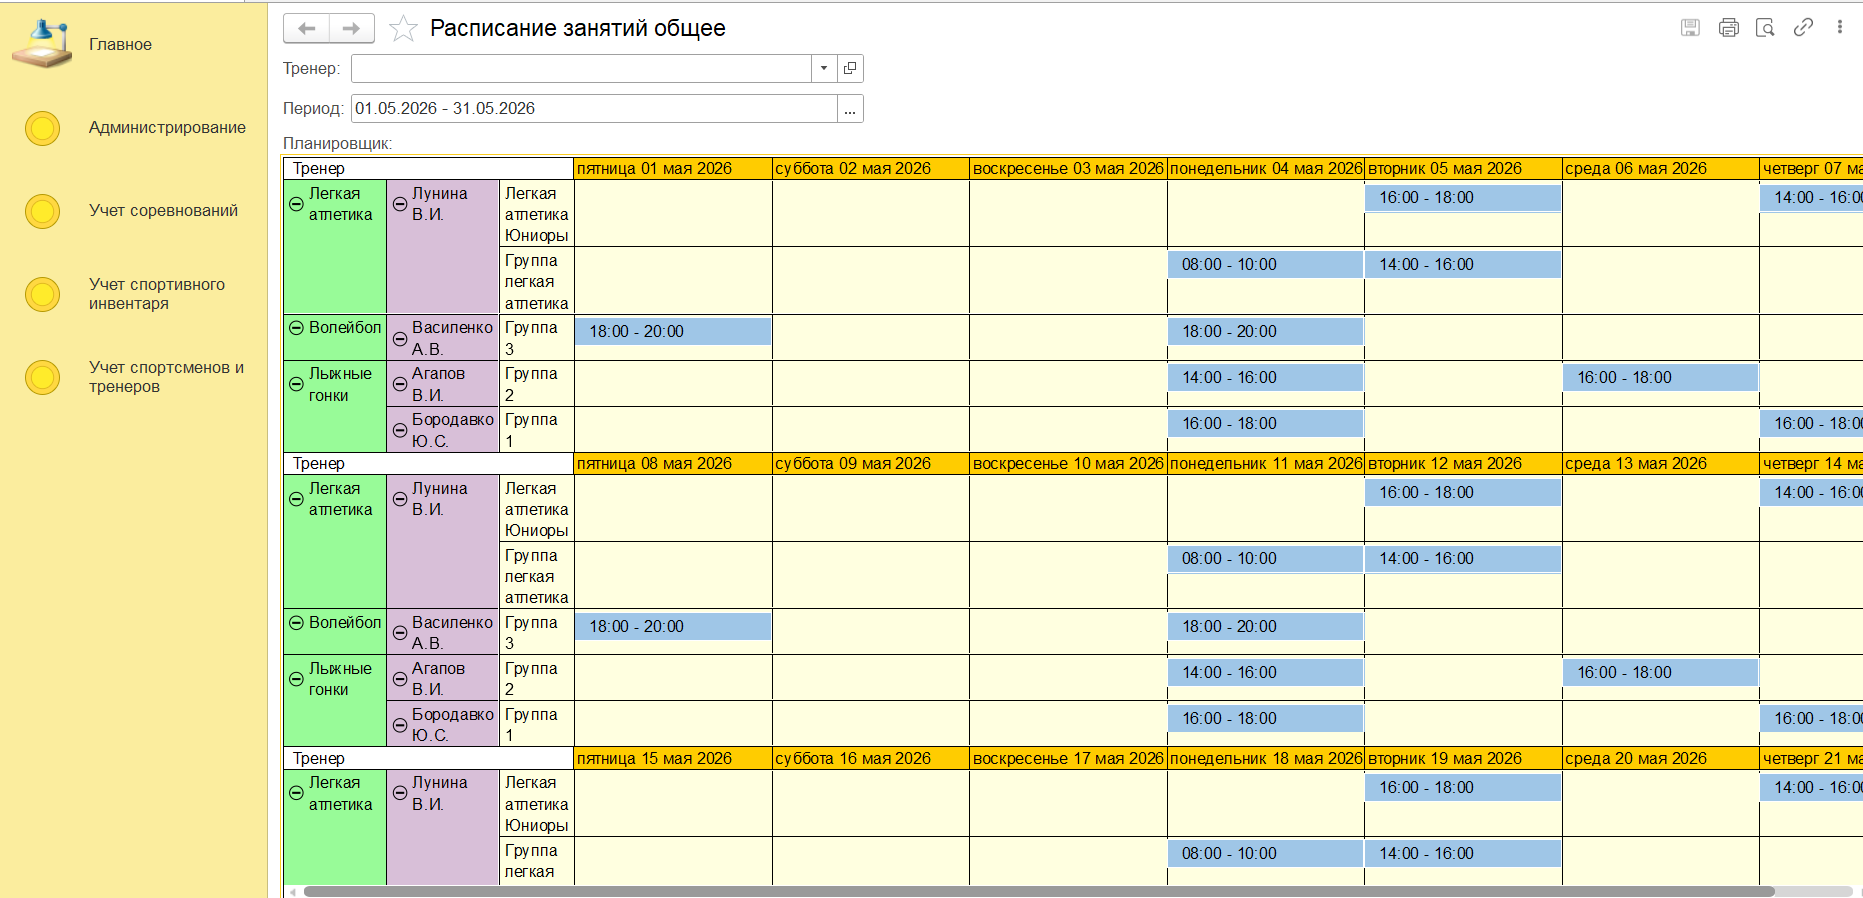
\includegraphics[width=0.9\textwidth]{images/raspis_zanatiy_rab_proeckt.png}
\end{center}
\begin{center}
	{Рисунок 4.1 - Отчет «Расписание занятий общее»}
\end{center}
\vspace{0.5cm}

\subsubsection{Тестовый сценарий: загрузка результатов соревнований из Excel}

\textbf{Предусловие:} система запущена, подготовлен файл Excel с результатами (12 строк с данными участников, дисциплин и результатов).

\textbf{Тестовый случай:} пользователь открывает документ «Результаты соревнований», нажимает «Заполнить из файла», выбирает подготовленный файл.

\textbf{Ожидаемый результат:} табличная часть документа заполнена данными из файла. Участники и дисциплины корректно сопоставлены со справочниками. Документ можно провести.

\textbf{Результат:} тест пройден успешно.

\vspace{1cm}
\begin{center}
	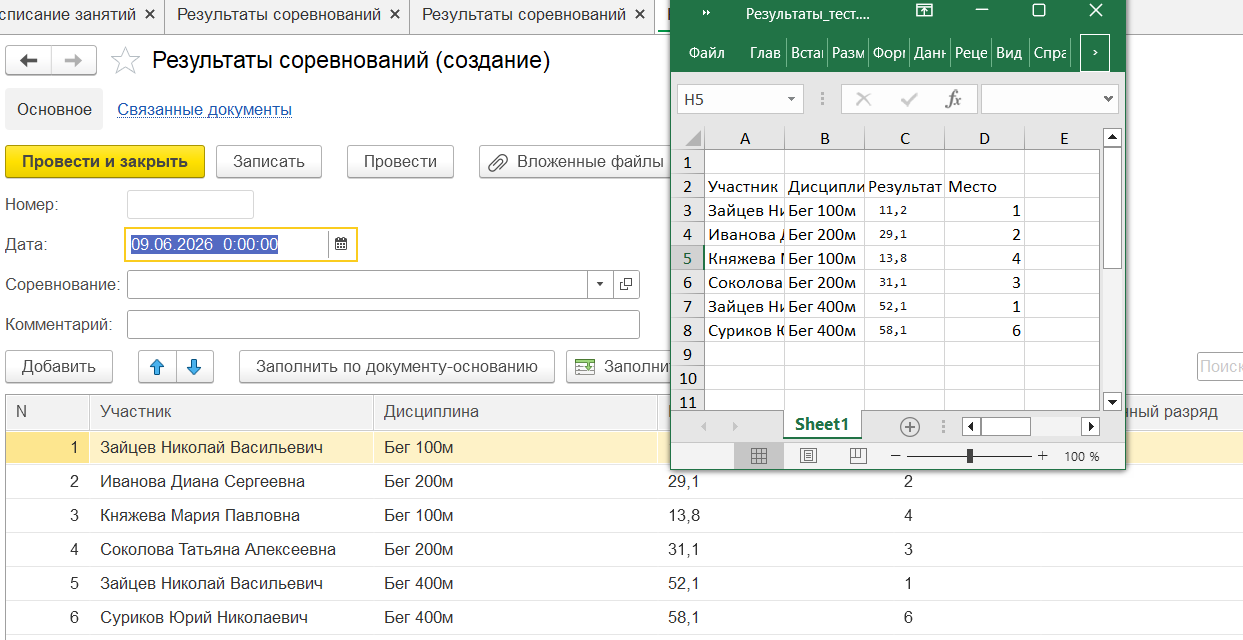
\includegraphics[width=0.9\textwidth]{images/rez_sorev1.png}
\end{center}
\begin{center}
	{Рисунок 4.2 - Форма документа «Результаты соревнований»}
\end{center}
\vspace{0.5cm}

\subsubsection{Тестовый сценарий: выдача инвентаря при недостатке на складе}

\textbf{Предусловие:} текущий остаток инвентаря «Палки Swix 155см» составляет 1 единицу.

\textbf{Тестовый случай:} пользователь создает документ «Выдача спортивного инвентаря», указывает инвентарь ««Палки Swix 155см», количество 5.

\textbf{Ожидаемый результат:} система выводит сообщение «Не удалось провести "Выдача спортивного инвентаря» В организации 1 из 5. Не хватает 4». Документ не проводится.

\textbf{Результат:} тест пройден успешно.

\vspace{1cm}
\begin{center}
	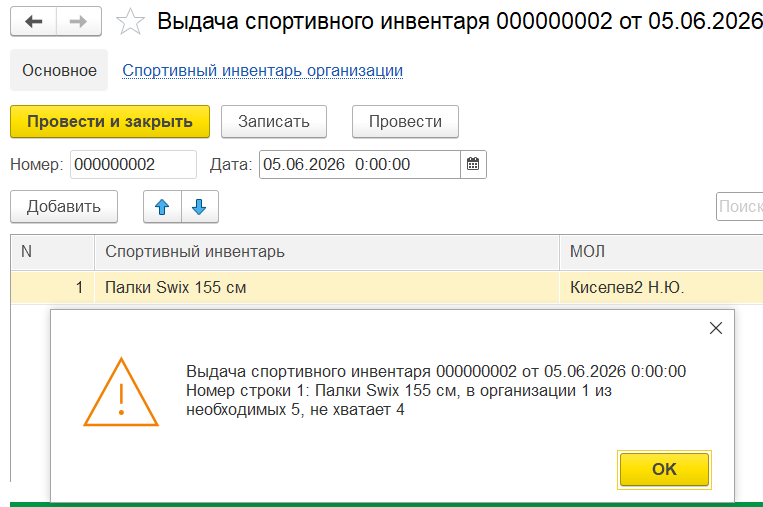
\includegraphics[width=0.9\textwidth]{images/vidacha.png}
\end{center}
\begin{center}
	{Рисунок 4.3 - «Выдача инвентаря»}
\end{center}
\vspace{0.5cm}

\subsubsection{Тестовый сценарий: формирование печатной формы приказа}

\textbf{Предусловие:} в системе имеется проведенный документ «Приказ о присвоении разряда» с заполненной табличной частью.

\textbf{Тестовый случай:} пользователь открывает документ и нажимает кнопку «Печать».

\textbf{Ожидаемый результат:} система формирует печатную форму приказа, содержащую наименование организации, номер и дату приказа, список спортсменов с видами спорта. Печатная форма открывается в режиме предварительного просмотра.

\textbf{Результат:} тест пройден успешно.

\vspace{1cm}
\begin{center}
	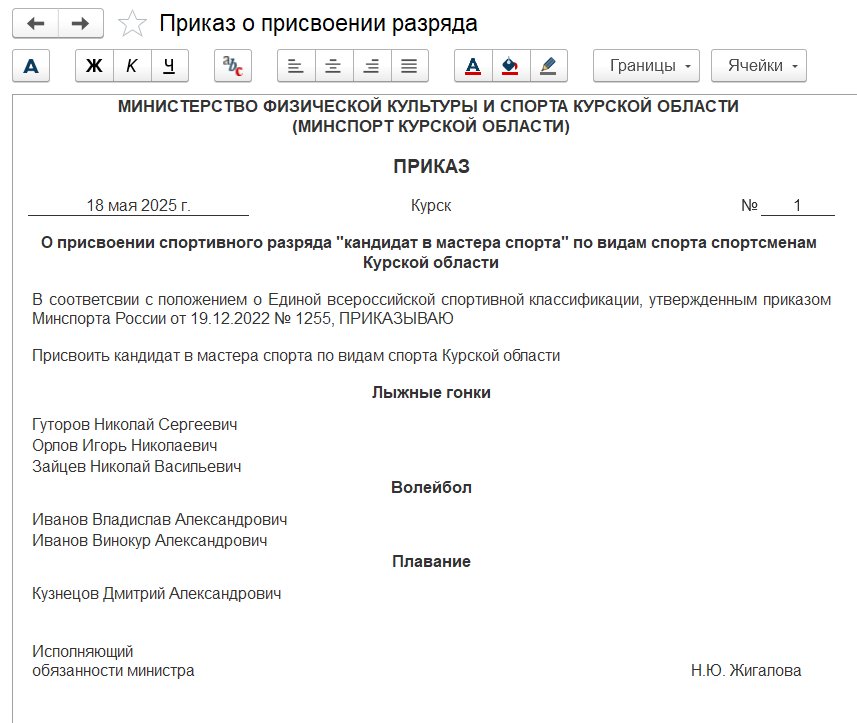
\includegraphics[width=0.9\textwidth]{images/prisvoenie_razr.png}
\end{center}
\begin{center}
	{Рисунок 4.4 - Печатная форма приказа о присвоении разряда}
\end{center}
\vspace{0.5cm}

\subsubsection{Тестовый сценарий: прикрепление файла к документу}

\textbf{Предусловие:} открыт документ «Соревнования», на диске имеется файл для прикрепления.

\textbf{Тестовый случай:} пользователь нажимает кнопку «Вложенные файлы», в открывшейся форме нажимает «Загрузить с диска» и выбирает файл с диска.

\textbf{Ожидаемый результат:} файл загружен в информационную базу и связан с документом. При повторном открытии формы вложенных файлов добавленный файл отображается в списке.

\textbf{Результат:} тест пройден успешно.

\vspace{1cm}
\begin{center}
	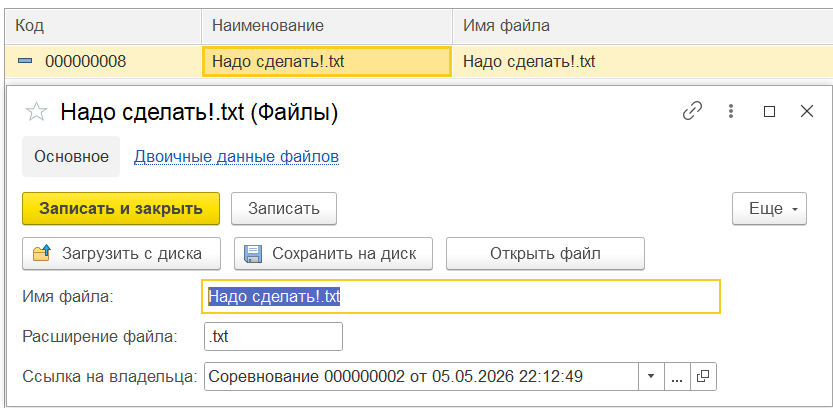
\includegraphics[width=0.9\textwidth]{images/fail.png}
\end{center}
\begin{center}
	{Рисунок 4.5 - Прикрепление файла}
\end{center}
\vspace{0.5cm}

\subsubsection{Тестовый сценарий: отправка почтового уведомления}

\textbf{Предусловие:} открыт документ «Соревнования» с участниками, у которых заполнены адреса электронной почты. В системе настроена учетная запись почты.

\textbf{Тестовый случай:} пользователь нажимает кнопку «Отправить напоминание по эл. почте».

\textbf{Ожидаемый результат:} система формирует письма и отправляет их участникам. Выводится сообщение о результате отправки.

\textbf{Результат:} тест пройден успешно (отправка выполнена, письма доставлены).

\vspace{1cm}
\begin{center}
	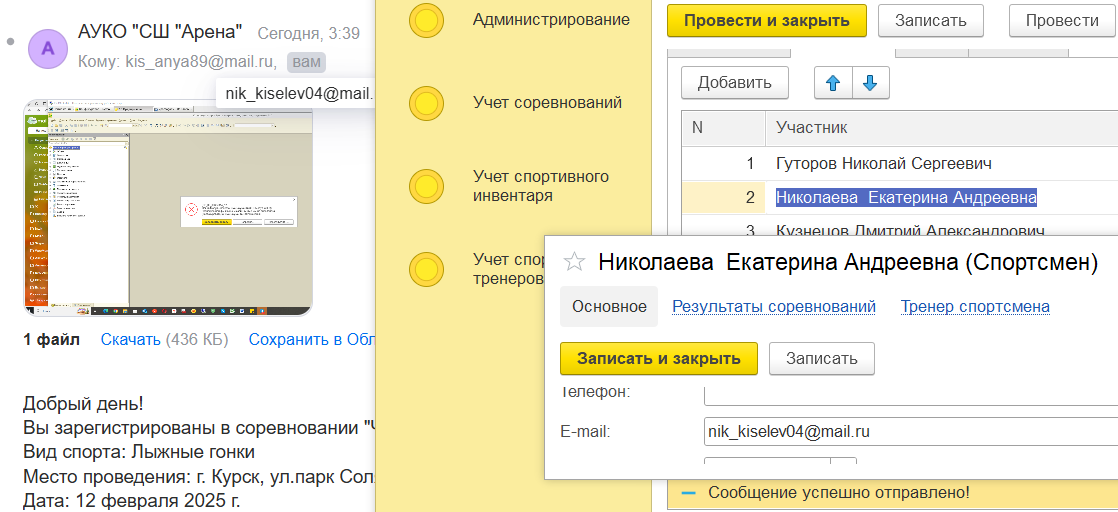
\includegraphics[width=0.9\textwidth]{images/uvedomlenie.png}
\end{center}
\begin{center}
	{Рисунок 4.6 - Отправка почтового уведомления}
\end{center}
\vspace{0.5cm}

\subsubsection{Тестовый сценарий: проверка разграничения прав доступа}

\textbf{Предусловие:} в системе создан пользователь с ролью «Тренер».

\textbf{Тестовый случай:} пользователь входит в систему под учетной записью тренера.

\textbf{Ожидаемый результат:} интерфейс отображает только подсистемы «Учет спортсменов и тренеров», «Учет соревнований» и «Учет спортивного инвентаря». Подсистема «Администрирование» не отображаются. 

\textbf{Результат:} тест пройден успешно.

\vspace{1cm}
\begin{center}
	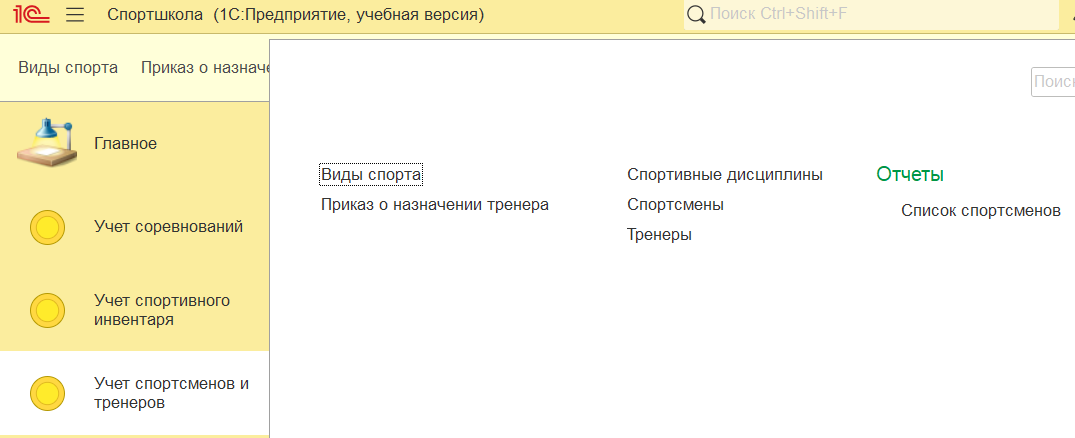
\includegraphics[width=0.9\textwidth]{images/vid_trener.png}
\end{center}
\begin{center}
	{Рисунок 4.7 - Интерфейс системы под ролью «Тренер»}
\end{center}
\vspace{0.5cm}

Рекомендуемая минимальная конфигурация компьютера: процессор с тактовой частотой от 2 ГГц, оперативная память от 4 ГБ, свободное дисковое пространство от 10 ГБ.